\documentclass[11pt]{article}

% Preamble

\usepackage[margin=1in]{geometry}
\usepackage{amsfonts, amsmath, amssymb}
\usepackage{fancyhdr, float, graphicx}
\usepackage[utf8]{inputenc} % Required for inputting international characters
\usepackage[T1]{fontenc} % Output font encoding for international characters
\usepackage{fouriernc} % Use the New Century Schoolbook font
\usepackage[nottoc, notlot, notlof]{tocbibind}
\usepackage{listings}
\usepackage{xcolor}
\usepackage{karnaugh-map}
% \usepackage[table,xcdraw]{xcolor}

\definecolor{codegreen}{rgb}{0,0.6,0}
\definecolor{codegray}{rgb}{0.5,0.5,0.5}
\definecolor{codepurple}{rgb}{0.58,0,0.82}
\definecolor{backcolour}{rgb}{0.95,0.95,0.92}

\lstdefinestyle{mystyle}{
    backgroundcolor=\color{backcolour},   
    commentstyle=\color{codegreen},
    keywordstyle=\color{magenta},
    numberstyle=\tiny\color{codegray},
    stringstyle=\color{codepurple},
    basicstyle=\ttfamily\footnotesize,
    breakatwhitespace=false,         
    breaklines=true,                 
    captionpos=b,                    
    keepspaces=true,                 
    numbers=left,                    
    numbersep=5pt,                  
    showspaces=false,                
    showstringspaces=false,
    showtabs=false,                  
    tabsize=2
}

\lstset{style=mystyle}

% Header and Footer
\pagestyle{fancy}
\fancyhead{}
\fancyfoot{}
\fancyhead[L]{\textit{\Large{DECA Assignment 4}}}
%\fancyhead[R]{\textit{something}}
\fancyfoot[C]{\thepage}
\renewcommand{\footrulewidth}{1pt}



% Other Doc Editing
% \parindent 0ex
%\renewcommand{\baselinestretch}{1.5}

\begin{document}

\begin{titlepage}
	\centering

	%---------------------------NAMES-------------------------------

	\huge\textsc{
		MIT World Peace University
	}\\

	\vspace{0.75\baselineskip} % space after Uni Name

	\LARGE{
		Digital Electronics and Computer Architecture\\
		Second Year B. Tech, Semester 3
	}

	\vfill % space after Sub Name

	%--------------------------TITLE-------------------------------

	\rule{\textwidth}{1.6pt}\vspace*{-\baselineskip}\vspace*{2pt}
	\rule{\textwidth}{0.6pt}
	\vspace{0.75\baselineskip} % Whitespace above the title



	\huge{\textsc{
			Design and Implementation of Asynchronous counters using\\ JK- Flip flop.
		}} \\



	\vspace{0.5\baselineskip} % Whitespace below the title
	\rule{\textwidth}{0.6pt}\vspace*{-\baselineskip}\vspace*{2.8pt}
	\rule{\textwidth}{1.6pt}

	\vspace{1\baselineskip} % Whitespace after the title block

	%--------------------------SUBTITLE --------------------------	

	\LARGE\textsc{
		Practical Report\\
		Assignment 4
	} % Subtitle or further description
	\vfill

	%--------------------------AUTHOR-------------------------------

	\vspace{0.5\baselineskip} % Whitespace before the editors

	\Large{
		Krishnaraj Thadesar \\
		Cyber Security and Forensics\\
		Batch A1, PA 20
	}


	\vspace{0.5\baselineskip} % Whitespace below the editor list
	\today

\end{titlepage}


\tableofcontents
\thispagestyle{empty}
\clearpage


\setcounter{page}{1}
\section{Objectives}
\begin{enumerate}
	\item To understand working of Modulo N counter using 7490(N>10).
\end{enumerate}

\section{Problem Statement}
Design and implement MOD 10, MOD 100 and MOD N counter using IC 7490.

\section{ICs Used}

\begin{enumerate}
	\item IC7490
	\item IC 7400
\end{enumerate}

\section{Platform Used}
Digital Trainer Kit

\section{Theory}

\subsection{IC 7490}

The IC 7490 is a decade counter. It is a 16 pin DIP IC. It has 4 inputs and 4 outputs. It has a carry output and a carry input. It has a clock input and a reset input. It has a preset input. It has a master reset

\subsection{Ripple counter IC-7490 (decade counter)}

IC 7490 is a 4 bit ripple type decade counter. It consists of four master or slave flip flops, which are internally connected to form a divide by two section and a divide by five section. Each section has a separate clock input to chnage the output states of the counter on a high to low clock transition. 

\subsection{Basic Structure of IC 7490}
IC 7490 is a 4-bit, ripple-type decade counter. It consists of four master/slave flip-flops, which are internally connected to form a divide-by-two section and a divide-by-five section.\\

Each section has a separate clock input to change the output states of the counter on a high-to-low clock transition. The output states do not change simultaneously due to the internal ripple delays. Therefore the decoded output signals are subject to decoding spikes and should not be used for clocks or strobes.\\

Since the output of the divide-by-two section is not internally connected to the succeeding stages, IC 7490 can be operated in various counting modes.\\

\section{Involved Truth Tables}

\subsection{NAND Gate}

\begin{table}[H]
	\begin{tabular}{|c|c|c|}
		\hline
		A & B & Result\\
		0 & 0 & 1 \\ \hline
		0 & 1 & 1 \\ \hline
		1 & 0 & 1 \\ \hline
		1 & 1 & 0 \\ \hline
		\end{tabular}
\end{table}
\subsection{Function table of IC7490}
\begin{figure}[H]
	\centering
	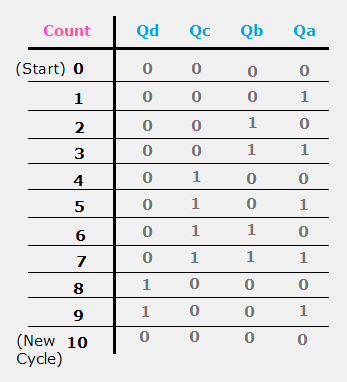
\includegraphics[scale = 0.85]{function table of 7490.png}
	\caption{Function Table of IC 7490}
\end{figure}



\subsection{JK Flip Flop Truth table}
\begin{figure}[H]
	\centering
	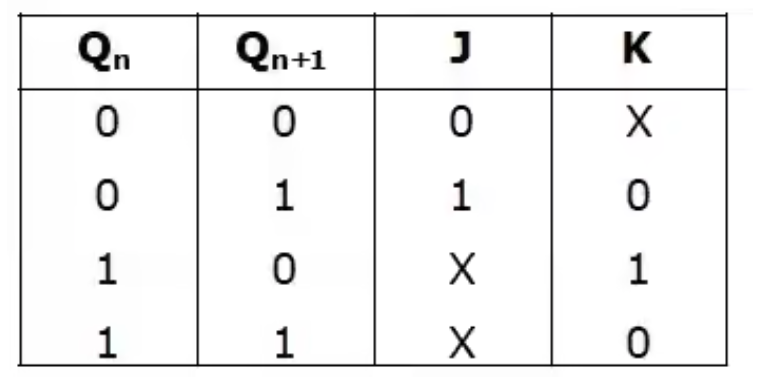
\includegraphics[scale = 0.5]{jk flip flop truth table.png}
	% \caption{Circuit diagram of a 3-bit synchronous counter - Down}
\end{figure}
\subsection{JK Flip Flop Excitation table}
\begin{figure}[H]
	\centering
	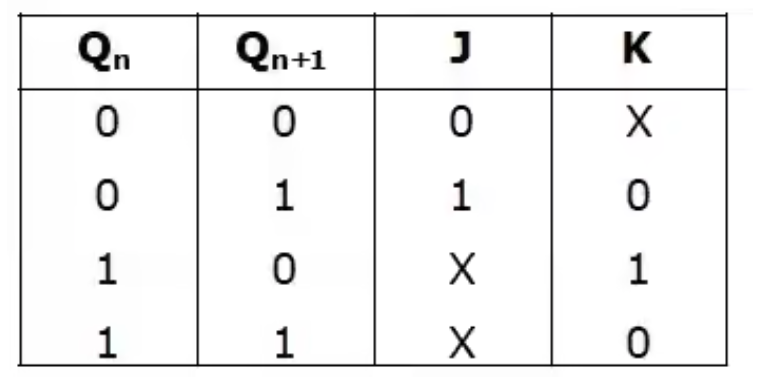
\includegraphics[scale = 0.5]{jk flip flop excitation table.png}
	% \caption{Circuit diagram of a 3-bit synchronous counter - Down}
\end{figure}
\subsection{JK Flip Flop Characteristic table}
\begin{figure}[H]
	\centering
	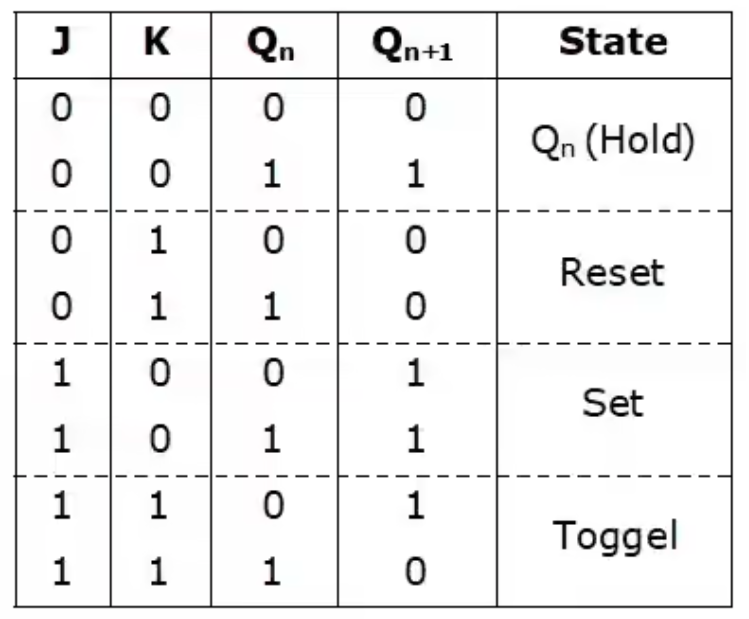
\includegraphics[scale = 0.5]{jk flip flop characteristic table.png}
	% \caption{Circuit diagram of a 3-bit synchronous counter - Down}
\end{figure}

\section{Pin Diagrams of ICs Used}

\subsection{Pin Diagram of IC7490}
\begin{figure}[H]
	\centering
	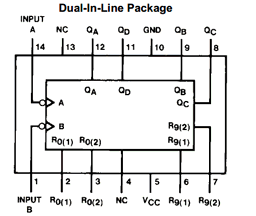
\includegraphics[scale = 1.5]{7490.png}
	\caption{Pin Diagram for IC 7490}
\end{figure}
\subsection{Pin Diagram of IC7400}
\begin{figure}[H]
	\centering
	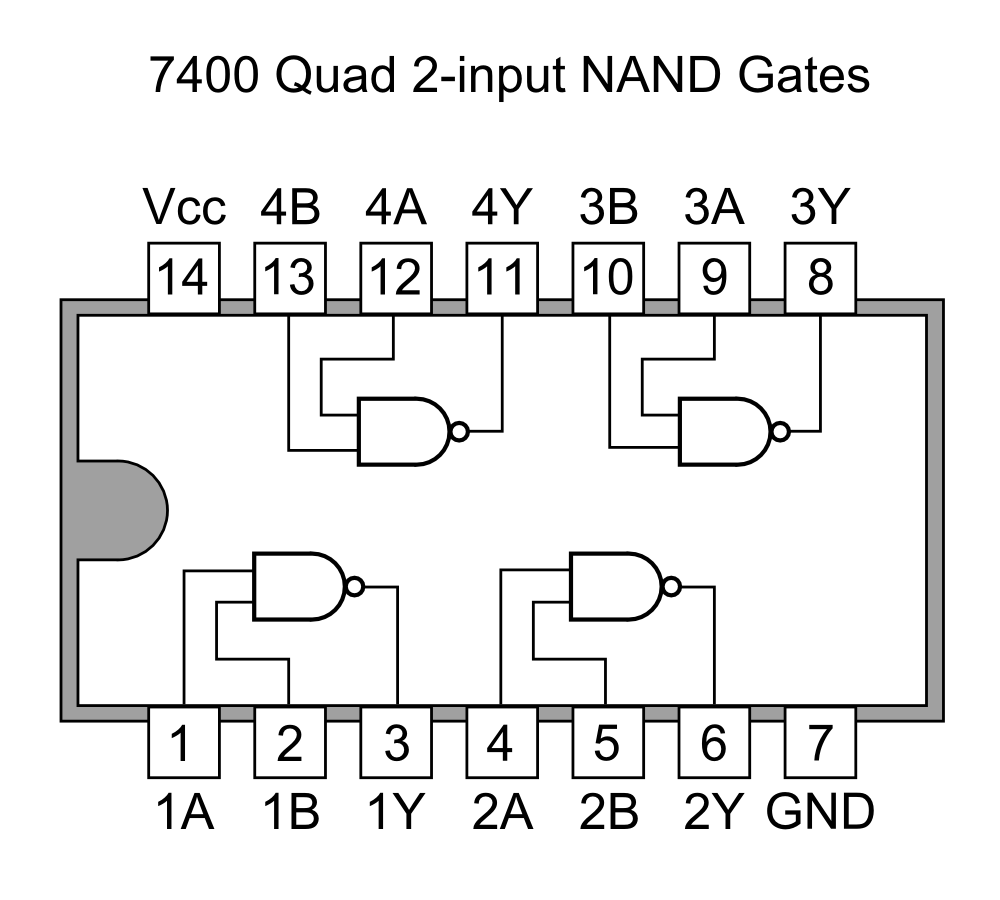
\includegraphics[scale = 0.25]{7400.png}
	\caption{Pin Diagram for IC 7400}
\end{figure}

\section{Design and Implementation}

\subsection{Circuit diagram of a Mod 10 Counter}
\begin{figure}[H]
	\centering
	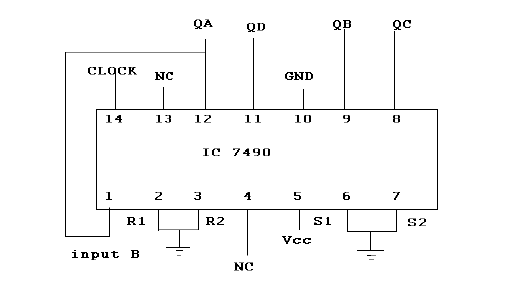
\includegraphics[scale = 0.5]{mod 10.png}
	\caption{Circuit diagram of a Mod 10 Counter}
\end{figure}

\subsection{Circuit diagram of a Mod 6 Counter}
\begin{figure}[H]
	\centering
	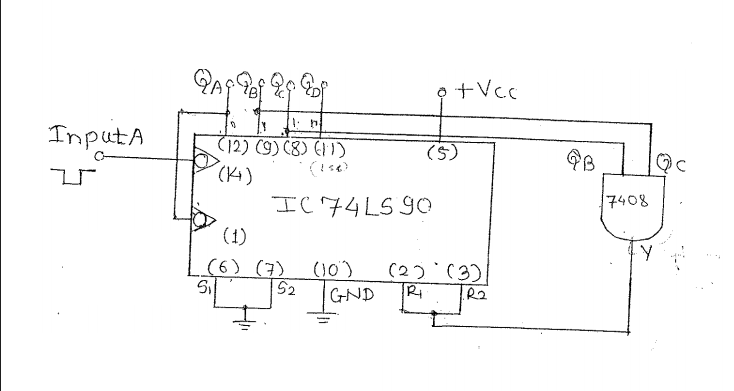
\includegraphics[scale = 0.5]{mod 6.png}
	\caption{Circuit diagram of a Mod 6 Counter}
\end{figure}

\subsection{Circuit diagram Mod 100 Counter}

\begin{figure}[H]
	\centering
	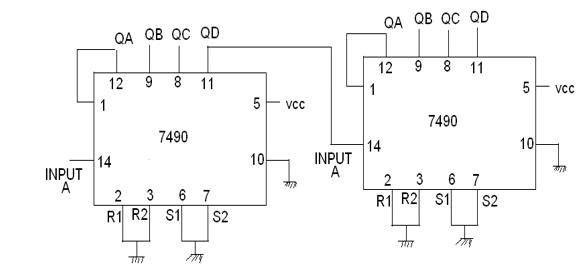
\includegraphics[scale = 0.45]{mod 100.png}
	\caption{Circuit diagram of Mod 100 Counter}
\end{figure}

\section{Conclusion}
\textit{Thus, we have learnt how to implement mod 10 and Mod 100 counters. Mod N counter was also learnt and implemented. Working of IC7490 was understood in detail. }

\pagebreak

\section{FAQs}

\begin{enumerate}
	\item What do you mean modulus Counter?\\
	The modulus of a counter is the number of states it can have. For example, a 4-bit counter can have 16 states. The modulus of a 4-bit counter is 16. Counters are generally classified as either synchronous or asynchronous. 
	\item Application of IC 7490?\\
	It is used in the design of asynchronous counters. It is also used in the design of asynchronous shift registers. It is also used in the design of asynchronous binary adders. It is also used in Automatic controller circuits. 
	
\end{enumerate}

\end{document}